\begin{figure}[h!]		
	\centering
   	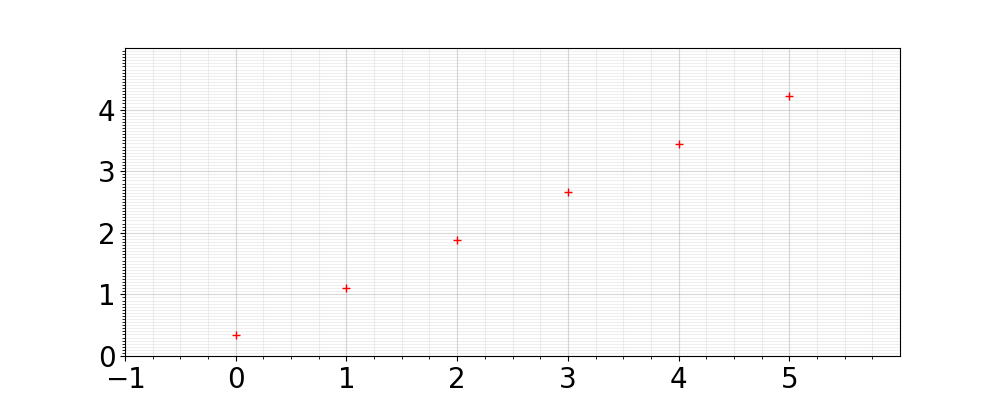
\includegraphics[width=8.0in]{pictures/picture_000.png}
  	\caption{Le coppie ordinate della tabella precedente, soddisfano l'equazione lineare $9y -7x - 3 = 0$ e quindi corrispondono a punti sul piano cartesiano che stanno tutti su una stessa retta. }
   	\label{fig:LibreOfficeCalc000}
\end{figure}
